% Author: Izaak Neutelings (June 2020)
\documentclass[border=3pt,tikz]{standalone}
\usetikzlibrary{calc}
\tikzset{>=latex} % for LaTeX arrow head

\newcommand\rightAngle[4]{
  \pgfmathanglebetweenpoints{\pgfpointanchor{#2}{center}}{\pgfpointanchor{#3}{center}}
  \coordinate (tmpRA) at ($(#2)+(\pgfmathresult+45:#4)$);
  \draw[blue!80!black] ($(#2)!(tmpRA)!(#1)$) -- (tmpRA) -- ($(#2)!(tmpRA)!(#3)$);
  %\fill[red] (tmpRA) circle(0.02);
}

\begin{document}


\begin{tikzpicture}
  \coordinate (O) at (0,0);
  \coordinate (X) at (1,0);
  \coordinate (Y) at (0,1);
  \draw (X) -- (O) -- (Y);
  \rightAngle{Y}{O}{X}{0.40}
\end{tikzpicture}


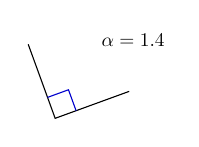
\begin{tikzpicture}
  \def\ang{20}
  \coordinate (O) at (0,0);
  \coordinate (X) at (\ang:1);
  \coordinate (Y) at (\ang+90:1);
  \draw (X) -- (O) -- (Y);
  \rightAngle{Y}{O}{X}{0.40}
  \node[scale=0.7] at (45:1.4) {$\alpha=\pgfmathresult$};
\end{tikzpicture}


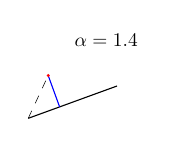
\begin{tikzpicture}
  \def\ang{20}
  \def\R{1.2}
  \coordinate (O) at (0,0);
  \coordinate (R) at (\ang:\R);
  \pgfmathanglebetweenpoints{\pgfpointanchor{O}{center}}{\pgfpointanchor{R}{center}}
  \draw (O) -- (R);
  \node[scale=0.7] at (45:1.4) {$\alpha=\pgfmathresult$};
  \coordinate (RA) at ($(O)+(\pgfmathresult+45:0.5*\R)$);
  \draw[dashed,very thin] (O) -- (RA);
  \draw[blue] ($(O)!(RA)!(R)$) -- (RA);
  \fill[red] (RA) circle(0.02);
\end{tikzpicture}


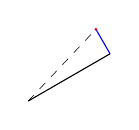
\begin{tikzpicture}
  \def\ang{30}
  \def\R{1.2}
  \coordinate (O) at (0,0);
  \coordinate (R) at (\ang:\R);
  \pgfmathanglebetweenpoints{\pgfpointanchor{O}{center}}{\pgfpointanchor{R}{center}}
  \draw (O) -- (R);
  \coordinate (RA) at ($(R)+(\pgfmathresult+90:0.3*\R)$);
  \coordinate (RA) at ($(R)+(\pgfmathresult+90:0.3*\R)$);
  \draw[dashed,very thin] (O) -- (RA);
  \draw[blue] ($(O)!(RA)!(R)$) -- (RA);
  \fill[red] (RA) circle(0.02);
\end{tikzpicture}


\end{document}